\documentclass{beamer}
\usepackage{beamerthemesplit}
\usepackage{wrapfig}
\usetheme{SPbGU}
\usepackage{pdfpages}
\usepackage{amsmath}
\usepackage{cmap} 
\usepackage[T2A]{fontenc} 
\usepackage[utf8]{inputenc}
\usepackage[english,russian]{babel}
\usepackage{indentfirst}
\usepackage{amsmath}
\usepackage{tikz}
\usepackage{dot2texi}
\usepackage{multirow}
\usepackage{fancyvrb}
\usepackage{graphicx}
\usepackage{array}
\usepackage{subcaption}
\usepackage[noend]{algpseudocode}
\usepackage{algorithm}
\usepackage{algorithmicx}
\usetikzlibrary{shapes,arrows}
\usepackage{fancyvrb}
\usepackage[normalem]{ulem} % для подчёркиваний uline
\newtheorem{rutheorem}{Теорема}
\newtheorem{ruproof}{Доказательство}
\newtheorem{rudefinition}{Определение}
\newtheorem{rulemma}{Лемма}
\beamertemplatenavigationsymbolsempty


\title[]{Диагностика синтаксических ошибок в динамически формируемом коде}
\subtitle[]{В рамках проекта лаборатории JetBrains}
% То, что в квадратных скобках, отображается в левом нижнем углу. 
\institute[СПбГУ]{
Санкт-Петербургский государственный университет \\
Кафедра системного программирования }

% То, что в квадратных скобках, отображается в левом нижнем углу.
\author[Азимов Рустам]{Азимов Рустам Шухратуллович, 444 группа \\
  % У научного руководителя должна быть указана научная степень
  \and  
    {\bfseries Научный руководитель:} м.и.т., ст.пр. С.В. Григорьев \\ 
  % Для курсовой не обязателен. Должна быть указана должность или ученая степень
  \and
    {\bfseries Рецензент:} программист "ИнтеллиДжей Лабс" Д.А. Авдюхин}

\date{17 мая 2016г.}

\definecolor{orange}{RGB}{179,36,31}

\begin{document}
{
% Лого университета или организации, отображается в шапке титульного листа
\begin{frame}
  \begin{center}
  {
\includegraphics[width=1cm]{pictures/SPbGU_Logo.png}}
  \end{center}
  \titlepage
\end{frame}
}

\begin{frame}[fragile]
  \transwipe[direction=90]
  \frametitle{Встроенные языки}
  \begin{itemize}
    \item Динамический SQL
      \begin{Verbatim}[commandchars=\\\{\}]
\textcolor{blue}{IF} @X = @Y
    \textcolor{blue}{SET} @TBL = \textcolor{orange}{' table1 '}
\textcolor{blue}{ELSE}
    \textcolor{blue}{SET} @TBL = \textcolor{orange}{'table2 '}
\textcolor{blue}{SET} @S = \textcolor{orange}{'SELECT x FROM'} + @TBL + \textcolor{orange}{'WHERE ISNULL(n,0) > 1'}
EXECUTE (@S)
       \end{Verbatim}
    \end{itemize}
\end{frame}

\begin{frame}[fragile]
	\transwipe[direction=90]
	\frametitle{Проблемы}
	\begin{itemize}
	    \item Динамически формируемые выражения -- код на некотором языке, который нужно соответствующим образом поддерживать и обрабатывать
        \begin{itemize}
    	    \item Ошибки в динамически формируемых выражениях обнаруживаются лишь во время выполнения
	        \item Поддержка в IDE
	        \item Реинжиниринг ПО, разработанного с использованием встроенных языков
	    \end{itemize}
    \end{itemize}
\end{frame}

            
\begin{frame}[fragile]
	\transwipe[direction=90]
	\frametitle{Статическая обработка встроенных языков}
	\begin{itemize}
	   \item Alvor, Java String Analyzer, PHP SA, Kyung-Goo Doh et al.
	    \begin{itemize}
	        \item Имеется дигностика синтаксических ошибок, но плохо расширяемы и не строят структурного представления кода
	    \end{itemize}
	   \item Ослабленный синтаксический анализ регулярной аппроксимации динамически формируемого кода в рамках проекта YaccConstructor
	    \begin{itemize}
	        \item Строит деревья вывода, хорошо расширяем, но синтаксические ошибки игнорируются
	        \item \textbf{Вход}: эталонная ДКС-грамматика $G$ и граф ДКА без 
$\epsilon$-переходов над алфавитом терминалов $G$
            \item \textbf{Выход}: конечное представление множества деревьев, соответствующих 
всем корректным цепочкам, принимаемым входным автоматом
	     \end{itemize}
    \end{itemize}
\end{frame}

\begin{frame}[fragile]
	\transwipe[direction=90]
	\frametitle{Пример}
		\begin{itemize}
	\item
\begin{Verbatim}[commandchars=\\\{\}]
\textcolor{blue}{IF} @X = @Y
    \textcolor{blue}{SET} @TBL = \textcolor{orange}{' table1 '}
\textcolor{blue}{ELSE}
    \textcolor{blue}{SET} @TBL = \textcolor{orange}{'table2 '}
\textcolor{blue}{SET} @S = \textcolor{orange}{'SELECT x FROM'} + @TBL + \textcolor{orange}{'WHERE ISNULL(n,0) > 1'}
EXECUTE (@S)
       \end{Verbatim}
     	\item Множество значений: \\ \{'SELECT x FROM table1 WHERE ISNULL(n,0) > 1' ; \\ \vspace{2pt} 'SELECT x FROMtable2 WHERE ISNULL(n,0) > 1'\}
    	\item Аппроксимация: 
            %\begin{center}
                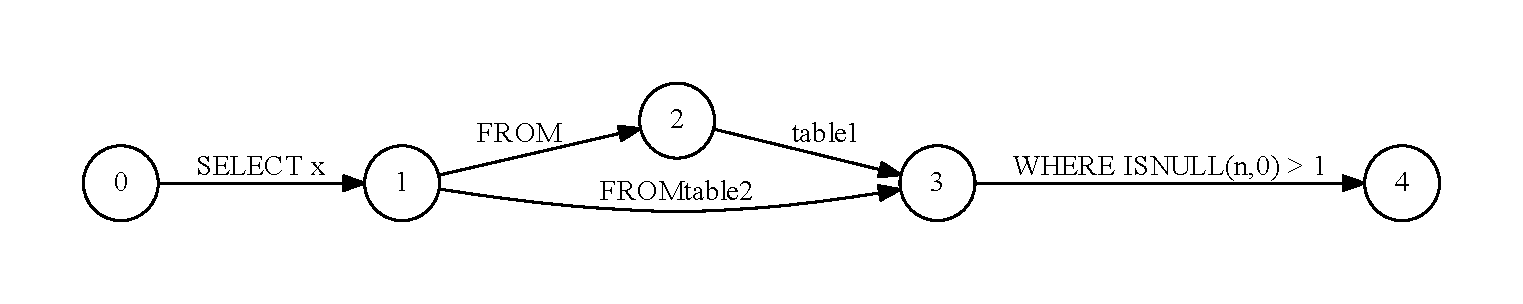
\includegraphics[width = 340pt,height=80pt]{pictures/SQLGraph.pdf}
            %\end{center}

	\end{itemize}

\end{frame}

\begin{frame}[fragile]
	\transwipe[direction=90]
	\frametitle{Синтаксические ошибки}
	\begin{itemize}
	    \item Алгоритмы LR семейства (LR, SLR, LALR)
    	\begin{itemize}
    		\item Читают входную строку слева направо
    		\item Строят стек состояний
        	\item Синтаксическая ошибка на символе, делающем невозможным дальнейшее построение стека состояний по таблице переходов грамматики
        \end{itemize}
        \item Обобщённый синтаксический анализ (GLR, RNGLR)
    	\begin{itemize}
    		\item Читает входную строку слева направо
    		\item Строит организованный в виде графа стек (GSS)
        	\item Синтаксическая ошибка на символе, делающем невозможным ни в одном направлении дальнейшее построение GSS состояний по таблице переходов грамматики
        \end{itemize}
    \end{itemize}
    \begin{itemize}
	    \item В обоих случаях синтаксическая ошибка на первом символе, делающем прочитанный префикс входной строки -- некорректным для рассматриваемой грамматики
    \end{itemize}
\end{frame}

% Обязательный слайд: четкая формулировка цели данной работы и постановка задачи
% Описание выносимых на защиту результатов, процесса или особенностей их достижения и т.д.
\begin{frame}
  \transwipe[direction=90]
  \frametitle{Постановка задачи}
  \textbf{Целью} работы является разработка механизма диагностики ошибок в ослабленном синтаксическом анализе регулярной аппроксимации динамически формируемого выражения 

  \textbf{Задачи}:
  \begin{itemize}
    \item Определить понятие синтаксической ошибки в терминах регулярной аппроксимации динамически формируемого выражения
    \item Разработать механизм диагностики ошибок в синтаксическом анализе регулярной аппроксимации динамически формируемого выражения
    \item Доказать корректность механизма
    \item Реализовать предложенный механизм на базе проекта YaccConstructor
    \item Провести экспериментальное исследование
  \end{itemize}
\end{frame}

\begin{frame}[fragile]
	\transwipe[direction=90]
	\frametitle{Понятие синтаксической ошибки}
    \begin{itemize}
        \item На вход вместо строки -- граф ДКА
        \item Вместо лексем -- ребра, нагруженные лексемами
    	\item Часть прочитанного входа не префикс строки, а путь в графе из начальной вершины (далее \uline{\textbf{префикс входного графа}})
    	\item Префикс входного графа \uline{\textbf{корректен}} для рассматриваемой грамматики $G$, если строка, образованная лексемами данного префикса, является корректным префиксом в грамматике $G$
    	\item Синтаксической ошибкой является ребро, делающее хотя бы один корректный префикс входного графа не корректным
	\end{itemize}
	\begin{center}
	            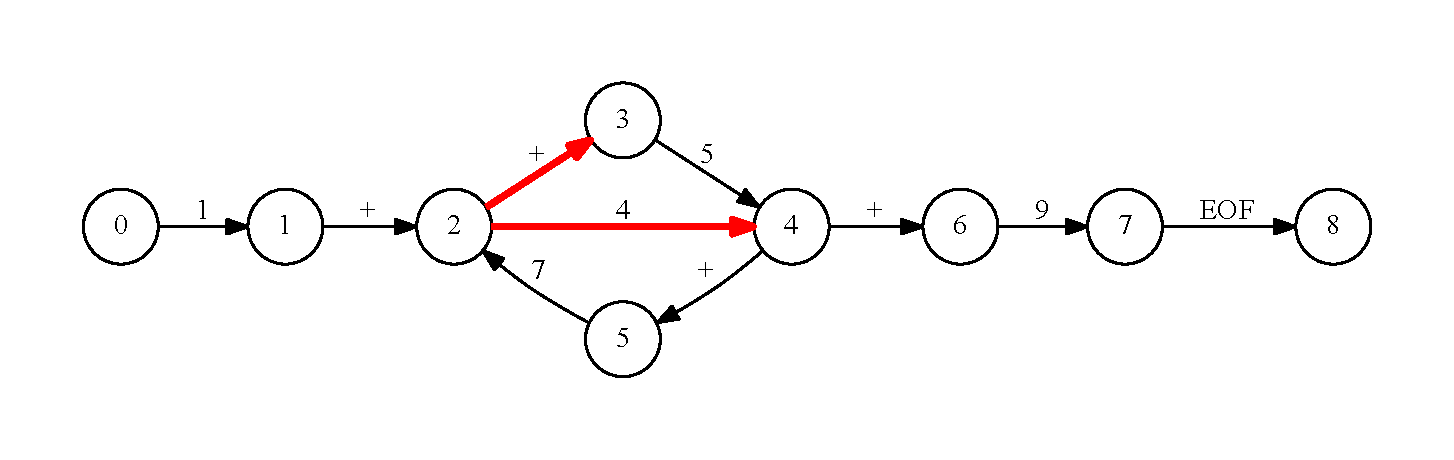
\includegraphics[width=340pt]{pictures/ErrorEdges.pdf}
	\end{center}
\end{frame}

\begin{frame}[fragile]
	\transwipe[direction=90]
	\frametitle{Механизм диагностики ошибок}
    \begin{itemize}
        \item Алгоритм построения префиксов --- модификация основного синтаксического анализа, дополнительно строящая для каждого GSS состояния все возможные корректные префиксы входного графа, ведущие в данное состояние
        \item Алгоритм диагностики ошибок --- с использованием обхода в глубину по входному графу, сравнивает множество построенных префиксов
        \item В результате -- создаются множества ребер $errors$ и $probErrors$, где все ребра из множества $errors$ являются ошибочными, а множество $errors \cup probErrors$ является аппроксимацией всех ошибочных ребер. Также для ребра $e$ указываются множества префиксов входного графа $errors[e]$ и $probErrors[e]$, где все префиксы из $errors[e]$ являются корректными для ребра $e$, а множество $errors[e] \cup probErrors[e]$ является аппроксимацией всех таких префиксов
    \end{itemize}
    
\end{frame}

\begin{frame}[fragile]
	\transwipe[direction=90]
	\frametitle{Пример работы алгоритма}
	\begin{itemize}
	    \item Грамматика:
	 
	 s ::= e
    
     e ::= Num + e | Num 
    
    \item
    Входной граф ДКА:
	            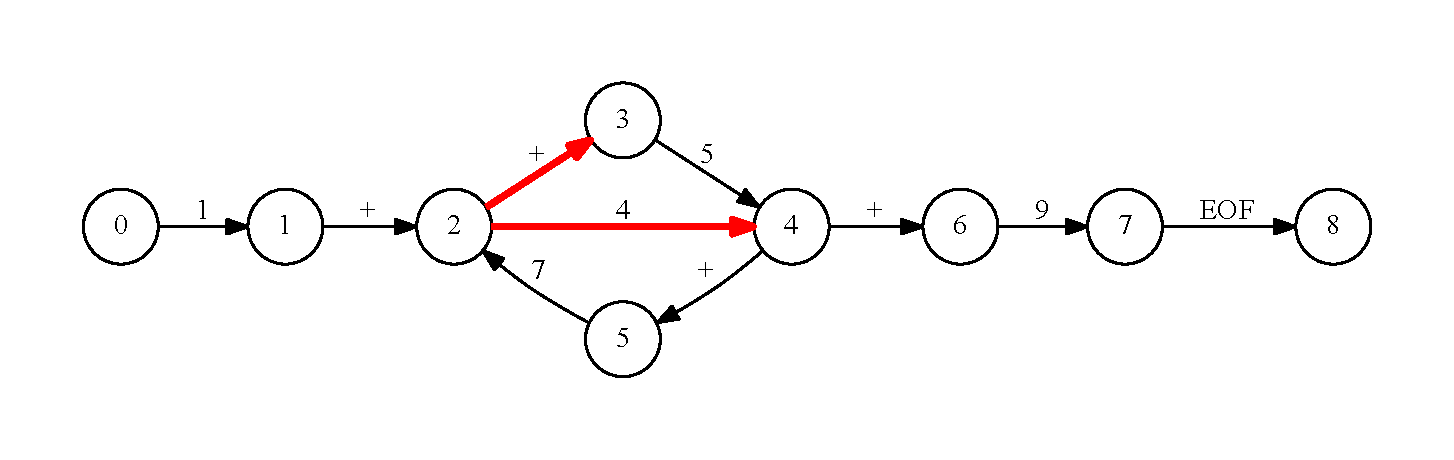
\includegraphics[width=340pt]{pictures/ErrorEdges.pdf}
    \end{itemize}
    
\end{frame}

\begin{frame}[fragile]
	\transwipe[direction=90]
	\frametitle{Пример работы алгоритма: префиксы}
	Синтаксическая ошибка:
	
	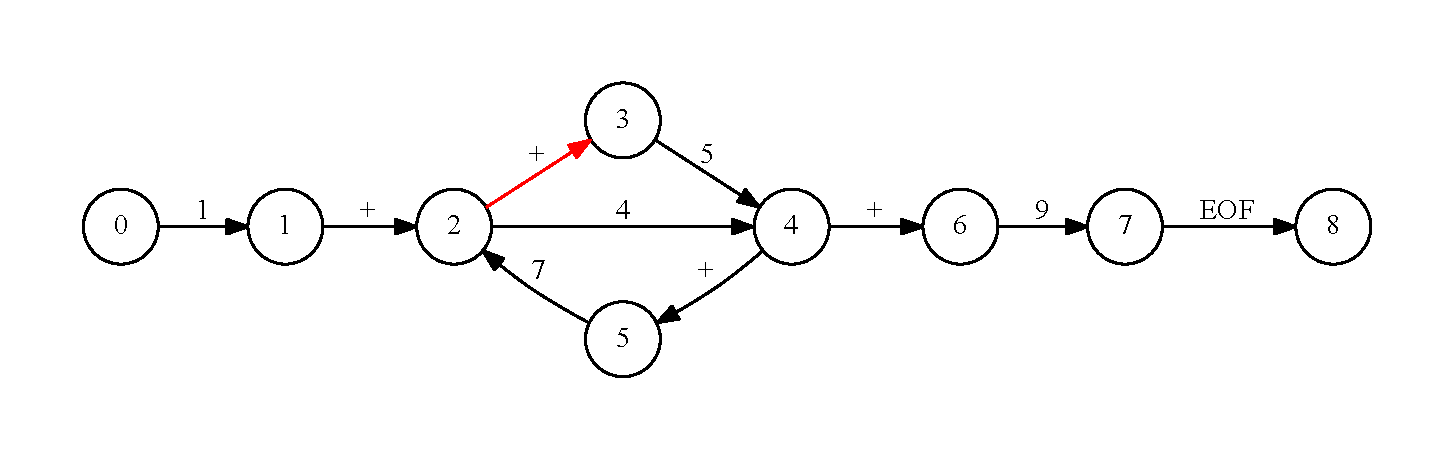
\includegraphics[width=340pt]{pictures/PlusErrorFull.pdf}
	
	Префиксы:
	
    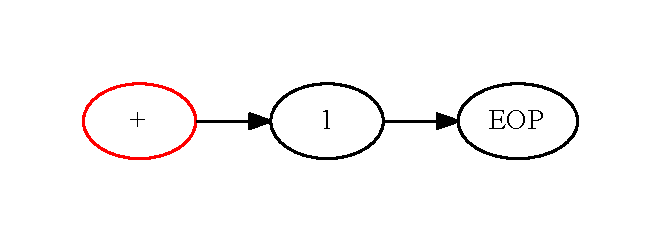
\includegraphics[width=250pt]{pictures/pluserror.pdf}
    
\end{frame}

\begin{frame}[fragile]
	\transwipe[direction=90]
	\frametitle{Пример работы алгоритма: префиксы}
	Синтаксическая ошибка:
	
	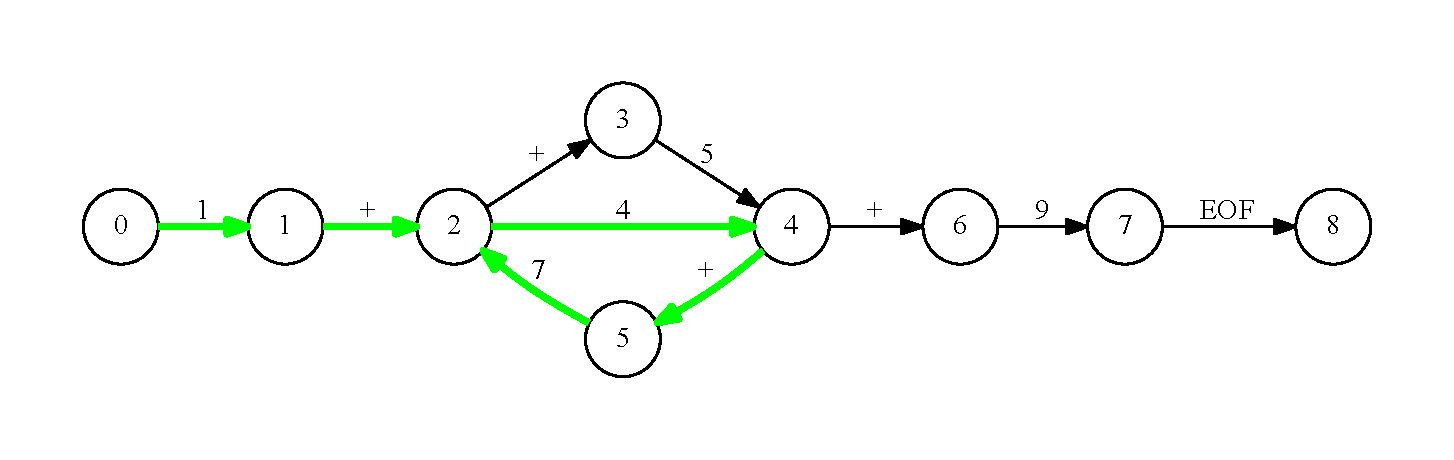
\includegraphics[width=340pt]{pictures/NumErrorFull.pdf}
	
	Префиксы:
	
    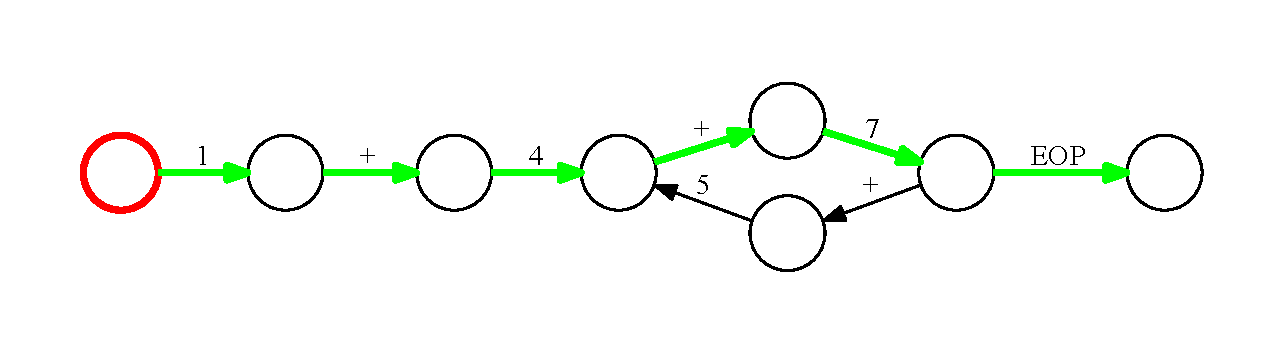
\includegraphics[width=340pt]{pictures/num4error.pdf}
    
\end{frame}

\begin{frame}[fragile]
  \transwipe[direction=90]
  \frametitle{Корректность механизма диагностики ошибок}
  \begin{rutheorem}[Корректность алгоритма построения префиксов]
    Для любого состояния GSS строятся все корректные префиксы входного графа, ведущие в данное состояние, и только они.
  \end{rutheorem}

  \begin{rutheorem}[Корректность алгоритма диагностики ошибок]
   Все ребра из построенного множества $errors$ являются ошибочными, а множество $errors \cup probErrors$ является аппроксимацией всех ошибочных ребер. Также для каждого ребра $e$, все префиксы входного графа из $errors[e]$ являются корректными для ребра $e$, а множество $errors[e] \cup probErrors[e]$ является аппроксимацией всех таких префиксов
  \end{rutheorem}
  
\end{frame}

%\begin{frame}[t]
 % \transwipe[direction=90]
  %\frametitle{Эксперимент}

%\end{frame}



\begin{frame}
  \transwipe[direction=90]
  \frametitle{Результаты}
  \begin{itemize}
    \item Определено понятие синтаксической ошибки в терминах регулярной аппроксимации динамически формируемого выражения
    \item Разработан алгоритм диагностики ошибок в синтаксическом анализе регулярной аппроксимации динамически формируемого выражения
    \item Выполнена реализация предложенного алгоритма на языке программирования F\# в рамках исследовательского проекта YaccConstructor
    \item Доказана корректность алгоритма
    \item Проведено экспериментальное исследование
  \end{itemize}
\end{frame}

\end{document}